\documentclass[twoside]{book}

% Packages required by doxygen
\usepackage{fixltx2e}
\usepackage{calc}
\usepackage{doxygen}
\usepackage[export]{adjustbox} % also loads graphicx
\usepackage{graphicx}
\usepackage[utf8]{inputenc}
\usepackage{makeidx}
\usepackage{multicol}
\usepackage{multirow}
\PassOptionsToPackage{warn}{textcomp}
\usepackage{textcomp}
\usepackage[nointegrals]{wasysym}
\usepackage[table]{xcolor}

% Font selection
\usepackage[T1]{fontenc}
\usepackage[scaled=.90]{helvet}
\usepackage{courier}
\usepackage{amssymb}
\usepackage{sectsty}
\renewcommand{\familydefault}{\sfdefault}
\allsectionsfont{%
  \fontseries{bc}\selectfont%
  \color{darkgray}%
}
\renewcommand{\DoxyLabelFont}{%
  \fontseries{bc}\selectfont%
  \color{darkgray}%
}
\newcommand{\+}{\discretionary{\mbox{\scriptsize$\hookleftarrow$}}{}{}}

% Page & text layout
\usepackage{geometry}
\geometry{%
  a4paper,%
  top=2.5cm,%
  bottom=2.5cm,%
  left=2.5cm,%
  right=2.5cm%
}
\tolerance=750
\hfuzz=15pt
\hbadness=750
\setlength{\emergencystretch}{15pt}
\setlength{\parindent}{0cm}
\setlength{\parskip}{0.2cm}
\makeatletter
\renewcommand{\paragraph}{%
  \@startsection{paragraph}{4}{0ex}{-1.0ex}{1.0ex}{%
    \normalfont\normalsize\bfseries\SS@parafont%
  }%
}
\renewcommand{\subparagraph}{%
  \@startsection{subparagraph}{5}{0ex}{-1.0ex}{1.0ex}{%
    \normalfont\normalsize\bfseries\SS@subparafont%
  }%
}
\makeatother

% Headers & footers
\usepackage{fancyhdr}
\pagestyle{fancyplain}
\fancyhead[LE]{\fancyplain{}{\bfseries\thepage}}
\fancyhead[CE]{\fancyplain{}{}}
\fancyhead[RE]{\fancyplain{}{\bfseries\leftmark}}
\fancyhead[LO]{\fancyplain{}{\bfseries\rightmark}}
\fancyhead[CO]{\fancyplain{}{}}
\fancyhead[RO]{\fancyplain{}{\bfseries\thepage}}
\fancyfoot[LE]{\fancyplain{}{}}
\fancyfoot[CE]{\fancyplain{}{}}
\fancyfoot[RE]{\fancyplain{}{\bfseries\scriptsize Generated on Wed Apr 22 2015 16\+:32\+:37 for A\+N\+S\+T\+\_\+\+Project by Doxygen }}
\fancyfoot[LO]{\fancyplain{}{\bfseries\scriptsize Generated on Wed Apr 22 2015 16\+:32\+:37 for A\+N\+S\+T\+\_\+\+Project by Doxygen }}
\fancyfoot[CO]{\fancyplain{}{}}
\fancyfoot[RO]{\fancyplain{}{}}
\renewcommand{\footrulewidth}{0.4pt}
\renewcommand{\chaptermark}[1]{%
  \markboth{#1}{}%
}
\renewcommand{\sectionmark}[1]{%
  \markright{\thesection\ #1}%
}

% Indices & bibliography
\usepackage{natbib}
\usepackage[titles]{tocloft}
\setcounter{tocdepth}{3}
\setcounter{secnumdepth}{5}
\makeindex

% Hyperlinks (required, but should be loaded last)
\usepackage{ifpdf}
\ifpdf
  \usepackage[pdftex,pagebackref=true]{hyperref}
\else
  \usepackage[ps2pdf,pagebackref=true]{hyperref}
\fi
\hypersetup{%
  colorlinks=true,%
  linkcolor=blue,%
  citecolor=blue,%
  unicode%
}

% Custom commands
\newcommand{\clearemptydoublepage}{%
  \newpage{\pagestyle{empty}\cleardoublepage}%
}


%===== C O N T E N T S =====

\begin{document}

% Titlepage & ToC
\hypersetup{pageanchor=false,
             bookmarks=true,
             bookmarksnumbered=true,
             pdfencoding=unicode
            }
\pagenumbering{roman}
\begin{titlepage}
\vspace*{7cm}
\begin{center}%
{\Large A\+N\+S\+T\+\_\+\+Project }\\
\vspace*{1cm}
{\large Generated by Doxygen 1.8.9.1}\\
\vspace*{0.5cm}
{\small Wed Apr 22 2015 16:32:37}\\
\end{center}
\end{titlepage}
\clearemptydoublepage
\tableofcontents
\clearemptydoublepage
\pagenumbering{arabic}
\hypersetup{pageanchor=true}

%--- Begin generated contents ---
\chapter{Hierarchical Index}
\section{Class Hierarchy}
This inheritance list is sorted roughly, but not completely, alphabetically\-:\begin{DoxyCompactList}
\item Mono\-Behaviour\begin{DoxyCompactList}
\item \contentsline{section}{Circle\-Script}{\pageref{class_circle_script}}{}
\item \contentsline{section}{Difficulty\-Script}{\pageref{class_difficulty_script}}{}
\item \contentsline{section}{G\-O\-Manager\-Script}{\pageref{class_g_o_manager_script}}{}
\item \contentsline{section}{hand\-Script}{\pageref{classhand_script}}{}
\item \contentsline{section}{H\-S\-Controller}{\pageref{class_h_s_controller}}{}
\item \contentsline{section}{Manager\-Script}{\pageref{class_manager_script}}{}
\item \contentsline{section}{menu\-Script}{\pageref{classmenu_script}}{}
\item \contentsline{section}{Pause\-Menu}{\pageref{class_pause_menu}}{}
\item \contentsline{section}{shooter\-Script}{\pageref{classshooter_script}}{}
\item \contentsline{section}{spawner\-Script}{\pageref{classspawner_script}}{}
\item \contentsline{section}{square\-Script}{\pageref{classsquare_script}}{}
\item \contentsline{section}{square\-Spawn\-Script}{\pageref{classsquare_spawn_script}}{}
\item \contentsline{section}{triangle\-Script}{\pageref{classtriangle_script}}{}
\end{DoxyCompactList}
\end{DoxyCompactList}

\chapter{Class Index}
\section{Class List}
Here are the classes, structs, unions and interfaces with brief descriptions\-:\begin{DoxyCompactList}
\item\contentsline{section}{\hyperlink{class_circle_script}{Circle\-Script} }{\pageref{class_circle_script}}{}
\item\contentsline{section}{\hyperlink{class_difficulty_script}{Difficulty\-Script} }{\pageref{class_difficulty_script}}{}
\item\contentsline{section}{\hyperlink{class_g_o_manager_script}{G\-O\-Manager\-Script} }{\pageref{class_g_o_manager_script}}{}
\item\contentsline{section}{\hyperlink{classhand_script}{hand\-Script} }{\pageref{classhand_script}}{}
\item\contentsline{section}{\hyperlink{class_h_s_controller}{H\-S\-Controller} }{\pageref{class_h_s_controller}}{}
\item\contentsline{section}{\hyperlink{class_manager_script}{Manager\-Script} }{\pageref{class_manager_script}}{}
\item\contentsline{section}{\hyperlink{classmenu_script}{menu\-Script} }{\pageref{classmenu_script}}{}
\item\contentsline{section}{\hyperlink{class_pause_menu}{Pause\-Menu} }{\pageref{class_pause_menu}}{}
\item\contentsline{section}{\hyperlink{classshooter_script}{shooter\-Script} }{\pageref{classshooter_script}}{}
\item\contentsline{section}{\hyperlink{classspawner_script}{spawner\-Script} }{\pageref{classspawner_script}}{}
\item\contentsline{section}{\hyperlink{classsquare_script}{square\-Script} }{\pageref{classsquare_script}}{}
\item\contentsline{section}{\hyperlink{classsquare_spawn_script}{square\-Spawn\-Script} }{\pageref{classsquare_spawn_script}}{}
\item\contentsline{section}{\hyperlink{classtriangle_script}{triangle\-Script} }{\pageref{classtriangle_script}}{}
\end{DoxyCompactList}

\chapter{Class Documentation}
\hypertarget{class_circle_script}{\section{Circle\-Script Class Reference}
\label{class_circle_script}\index{Circle\-Script@{Circle\-Script}}
}
Inheritance diagram for Circle\-Script\-:\begin{figure}[H]
\begin{center}
\leavevmode
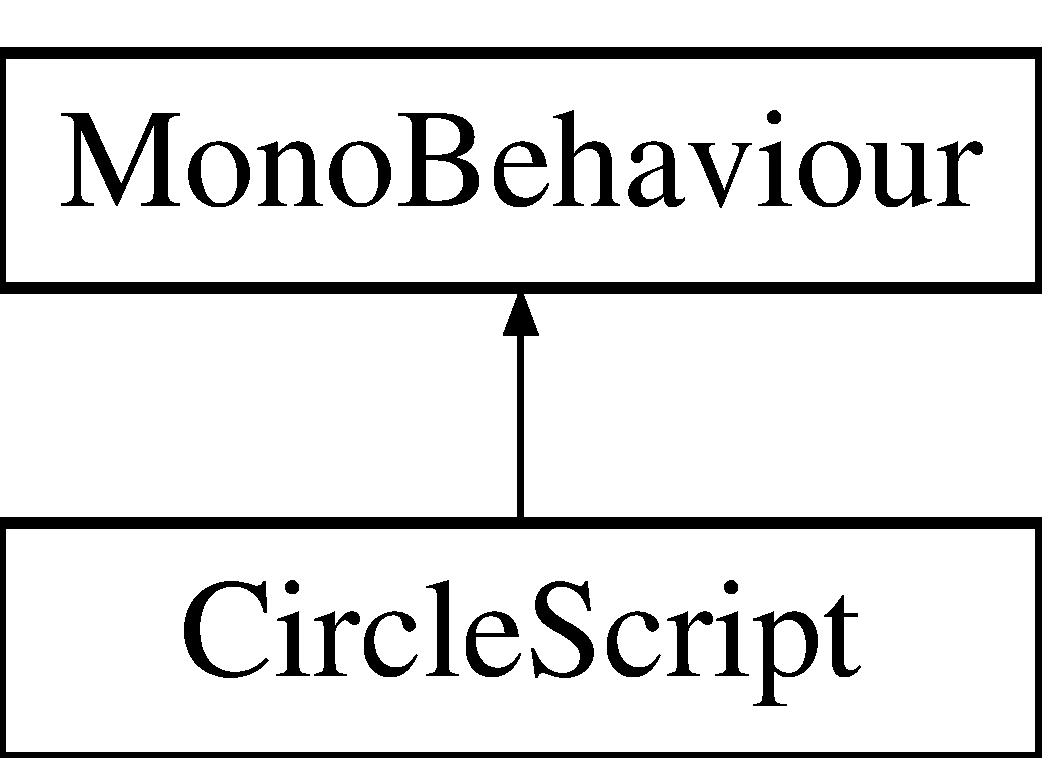
\includegraphics[height=2.000000cm]{class_circle_script}
\end{center}
\end{figure}
\subsection*{Public Member Functions}
\begin{DoxyCompactItemize}
\item 
void \hyperlink{class_circle_script_a1d1b1b39ff03be1b31fa855760e2f704}{On\-Trigger\-Enter2\-D} (Collider2\-D obj)
\item 
void \hyperlink{class_circle_script_ac2f21c8ce3074c924eece8d688a5a87f}{On\-Became\-Invisible} ()
\end{DoxyCompactItemize}
\subsection*{Public Attributes}
\begin{DoxyCompactItemize}
\item 
Vector2 \hyperlink{class_circle_script_a4b8a0a38630b44c7e210b8b6be2549c2}{speed} = new Vector2(-\/20,0)
\item 
\hyperlink{class_manager_script}{Manager\-Script} \hyperlink{class_circle_script_ac766a11165e1111c478837fae3df9c19}{manager\-Script}
\begin{DoxyCompactList}\small\item\em Set the speed. \end{DoxyCompactList}\end{DoxyCompactItemize}
\subsection*{Private Member Functions}
\begin{DoxyCompactItemize}
\item 
void \hyperlink{class_circle_script_a79d3a6c4e26f7235eff64bcb1bb8af99}{Start} ()
\end{DoxyCompactItemize}


\subsection{Detailed Description}
This script is used by the Circle objects in the game. This script deals with the collision detection of the Square objects. 

\subsection{Member Function Documentation}
\hypertarget{class_circle_script_ac2f21c8ce3074c924eece8d688a5a87f}{\index{Circle\-Script@{Circle\-Script}!On\-Became\-Invisible@{On\-Became\-Invisible}}
\index{On\-Became\-Invisible@{On\-Became\-Invisible}!CircleScript@{Circle\-Script}}
\subsubsection[{On\-Became\-Invisible}]{\setlength{\rightskip}{0pt plus 5cm}void Circle\-Script.\-On\-Became\-Invisible (
\begin{DoxyParamCaption}
{}
\end{DoxyParamCaption}
)\hspace{0.3cm}{\ttfamily [inline]}}}\label{class_circle_script_ac2f21c8ce3074c924eece8d688a5a87f}
This function destroys the object when it leaves the screen. Triangles will destroy our game\-Objects \hypertarget{class_circle_script_a1d1b1b39ff03be1b31fa855760e2f704}{\index{Circle\-Script@{Circle\-Script}!On\-Trigger\-Enter2\-D@{On\-Trigger\-Enter2\-D}}
\index{On\-Trigger\-Enter2\-D@{On\-Trigger\-Enter2\-D}!CircleScript@{Circle\-Script}}
\subsubsection[{On\-Trigger\-Enter2\-D}]{\setlength{\rightskip}{0pt plus 5cm}void Circle\-Script.\-On\-Trigger\-Enter2\-D (
\begin{DoxyParamCaption}
\item[{Collider2\-D}]{obj}
\end{DoxyParamCaption}
)\hspace{0.3cm}{\ttfamily [inline]}}}\label{class_circle_script_a1d1b1b39ff03be1b31fa855760e2f704}
This function handles the collision detection of the Circle objects. This function is called when a collision with a Triangle object is detected. Handles removal of both Circle and Triangle objects and adds to the score. 
\begin{DoxyParams}{Parameters}
{\em obj} & the object that collided with the Circle \\
\hline
\end{DoxyParams}
If there are triangles present...

Triangles must be capable of destroying our squares. \hypertarget{class_circle_script_a79d3a6c4e26f7235eff64bcb1bb8af99}{\index{Circle\-Script@{Circle\-Script}!Start@{Start}}
\index{Start@{Start}!CircleScript@{Circle\-Script}}
\subsubsection[{Start}]{\setlength{\rightskip}{0pt plus 5cm}void Circle\-Script.\-Start (
\begin{DoxyParamCaption}
{}
\end{DoxyParamCaption}
)\hspace{0.3cm}{\ttfamily [inline]}, {\ttfamily [private]}}}\label{class_circle_script_a79d3a6c4e26f7235eff64bcb1bb8af99}
This function runs when the script is first initialized. The function sets the speed of the circle and then gets the object that has the tag \hyperlink{class_manager_script}{Manager\-Script}. Initializing velocity in terms of speed.

If object exists. 

\subsection{Member Data Documentation}
\hypertarget{class_circle_script_ac766a11165e1111c478837fae3df9c19}{\index{Circle\-Script@{Circle\-Script}!manager\-Script@{manager\-Script}}
\index{manager\-Script@{manager\-Script}!CircleScript@{Circle\-Script}}
\subsubsection[{manager\-Script}]{\setlength{\rightskip}{0pt plus 5cm}{\bf Manager\-Script} Circle\-Script.\-manager\-Script}}\label{class_circle_script_ac766a11165e1111c478837fae3df9c19}


Set the speed. 

The variable to the \hyperlink{class_manager_script}{Manager\-Script} instance. \hypertarget{class_circle_script_a4b8a0a38630b44c7e210b8b6be2549c2}{\index{Circle\-Script@{Circle\-Script}!speed@{speed}}
\index{speed@{speed}!CircleScript@{Circle\-Script}}
\subsubsection[{speed}]{\setlength{\rightskip}{0pt plus 5cm}Vector2 Circle\-Script.\-speed = new Vector2(-\/20,0)}}\label{class_circle_script_a4b8a0a38630b44c7e210b8b6be2549c2}
The variable to store the speed of the circle. 

The documentation for this class was generated from the following file\-:\begin{DoxyCompactItemize}
\item 
A\-O\-T2/\-Assets/\-Scripts/\hyperlink{_circle_script_8cs}{Circle\-Script.\-cs}\end{DoxyCompactItemize}

\hypertarget{class_difficulty_script}{\section{Difficulty\-Script Class Reference}
\label{class_difficulty_script}\index{Difficulty\-Script@{Difficulty\-Script}}
}
Inheritance diagram for Difficulty\-Script\-:\begin{figure}[H]
\begin{center}
\leavevmode
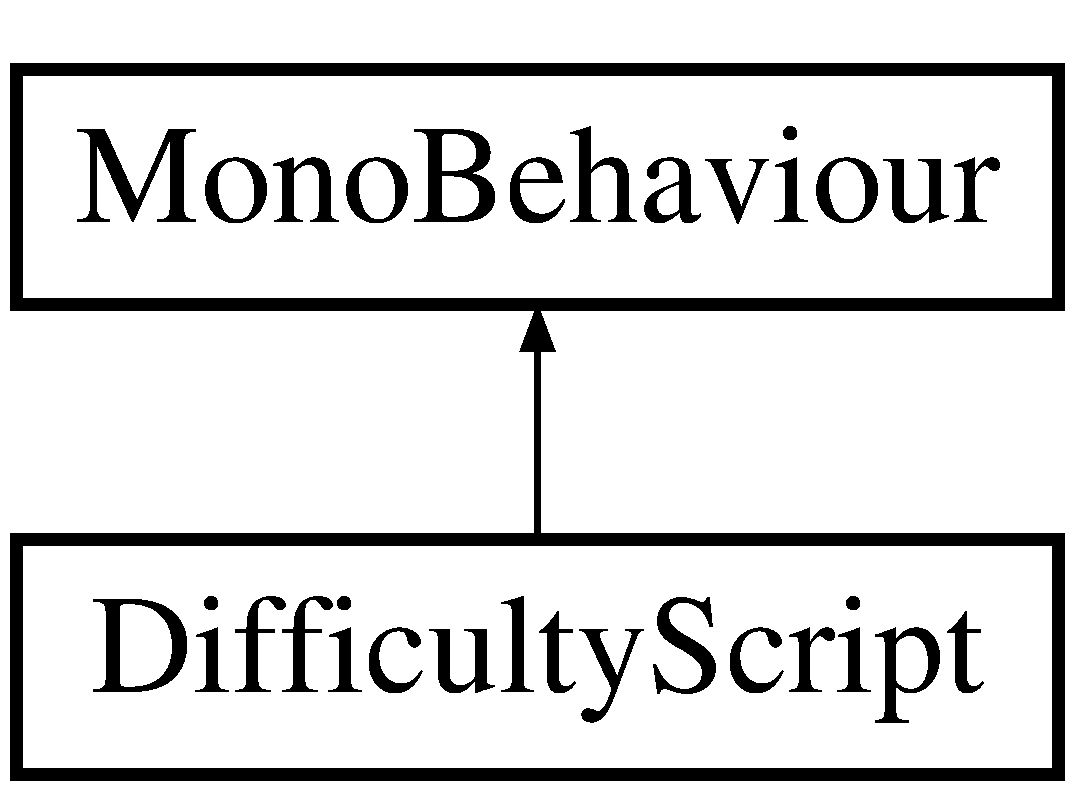
\includegraphics[height=2.000000cm]{class_difficulty_script}
\end{center}
\end{figure}
\subsection*{Public Member Functions}
\begin{DoxyCompactItemize}
\item 
void \hyperlink{class_difficulty_script_ad8913d5e49546c27235a5237a8338a48}{Easy} ()
\begin{DoxyCompactList}\small\item\em This method changes difficulty to Easy. \end{DoxyCompactList}\item 
void \hyperlink{class_difficulty_script_aaa1f844ba07536daad09d0d953f15ee9}{Medium} ()
\begin{DoxyCompactList}\small\item\em Changes difficulty to Medium. \end{DoxyCompactList}\item 
void \hyperlink{class_difficulty_script_a114d050f8e4c4bc684728ea9d4f143d1}{Hard} ()
\begin{DoxyCompactList}\small\item\em Changes difficulty to Hard. \end{DoxyCompactList}\end{DoxyCompactItemize}
\subsection*{Public Attributes}
\begin{DoxyCompactItemize}
\item 
Text \hyperlink{class_difficulty_script_a6cf366e11e24688822b51ad02a591d12}{this\-Text}
\begin{DoxyCompactList}\small\item\em Difficulty will be adjusted based on a few integers. \end{DoxyCompactList}\item 
Text \hyperlink{class_difficulty_script_ac35d383f05d94d0388dae2aa9544aeec}{other\-Text1}
\item 
Text \hyperlink{class_difficulty_script_a88e0b2f1fdb864f25e32c7945467befa}{other\-Text2}
\end{DoxyCompactItemize}
\subsection*{Static Public Attributes}
\begin{DoxyCompactItemize}
\item 
static int \hyperlink{class_difficulty_script_a1a931c1e4bc7c3465dc3e6a0bb4ac9d8}{difficulty}
\end{DoxyCompactItemize}
\subsection*{Private Member Functions}
\begin{DoxyCompactItemize}
\item 
void \hyperlink{class_difficulty_script_a4238d7fde036dfd58b2e1087ce40d176}{Start} ()
\item 
void \hyperlink{class_difficulty_script_ad8272764f6c0db30baf4b0f09b225ab7}{color\-Changes} ()
\begin{DoxyCompactList}\small\item\em This method handles any color changes the user wishes to impose. \end{DoxyCompactList}\end{DoxyCompactItemize}


\subsection{Member Function Documentation}
\hypertarget{class_difficulty_script_ad8272764f6c0db30baf4b0f09b225ab7}{\index{Difficulty\-Script@{Difficulty\-Script}!color\-Changes@{color\-Changes}}
\index{color\-Changes@{color\-Changes}!DifficultyScript@{Difficulty\-Script}}
\subsubsection[{color\-Changes}]{\setlength{\rightskip}{0pt plus 5cm}void Difficulty\-Script.\-color\-Changes (
\begin{DoxyParamCaption}
{}
\end{DoxyParamCaption}
)\hspace{0.3cm}{\ttfamily [inline]}, {\ttfamily [private]}}}\label{class_difficulty_script_ad8272764f6c0db30baf4b0f09b225ab7}


This method handles any color changes the user wishes to impose. 

\hypertarget{class_difficulty_script_ad8913d5e49546c27235a5237a8338a48}{\index{Difficulty\-Script@{Difficulty\-Script}!Easy@{Easy}}
\index{Easy@{Easy}!DifficultyScript@{Difficulty\-Script}}
\subsubsection[{Easy}]{\setlength{\rightskip}{0pt plus 5cm}void Difficulty\-Script.\-Easy (
\begin{DoxyParamCaption}
{}
\end{DoxyParamCaption}
)\hspace{0.3cm}{\ttfamily [inline]}}}\label{class_difficulty_script_ad8913d5e49546c27235a5237a8338a48}


This method changes difficulty to Easy. 

\hypertarget{class_difficulty_script_a114d050f8e4c4bc684728ea9d4f143d1}{\index{Difficulty\-Script@{Difficulty\-Script}!Hard@{Hard}}
\index{Hard@{Hard}!DifficultyScript@{Difficulty\-Script}}
\subsubsection[{Hard}]{\setlength{\rightskip}{0pt plus 5cm}void Difficulty\-Script.\-Hard (
\begin{DoxyParamCaption}
{}
\end{DoxyParamCaption}
)\hspace{0.3cm}{\ttfamily [inline]}}}\label{class_difficulty_script_a114d050f8e4c4bc684728ea9d4f143d1}


Changes difficulty to Hard. 

\hypertarget{class_difficulty_script_aaa1f844ba07536daad09d0d953f15ee9}{\index{Difficulty\-Script@{Difficulty\-Script}!Medium@{Medium}}
\index{Medium@{Medium}!DifficultyScript@{Difficulty\-Script}}
\subsubsection[{Medium}]{\setlength{\rightskip}{0pt plus 5cm}void Difficulty\-Script.\-Medium (
\begin{DoxyParamCaption}
{}
\end{DoxyParamCaption}
)\hspace{0.3cm}{\ttfamily [inline]}}}\label{class_difficulty_script_aaa1f844ba07536daad09d0d953f15ee9}


Changes difficulty to Medium. 

\hypertarget{class_difficulty_script_a4238d7fde036dfd58b2e1087ce40d176}{\index{Difficulty\-Script@{Difficulty\-Script}!Start@{Start}}
\index{Start@{Start}!DifficultyScript@{Difficulty\-Script}}
\subsubsection[{Start}]{\setlength{\rightskip}{0pt plus 5cm}void Difficulty\-Script.\-Start (
\begin{DoxyParamCaption}
{}
\end{DoxyParamCaption}
)\hspace{0.3cm}{\ttfamily [inline]}, {\ttfamily [private]}}}\label{class_difficulty_script_a4238d7fde036dfd58b2e1087ce40d176}


\subsection{Member Data Documentation}
\hypertarget{class_difficulty_script_a1a931c1e4bc7c3465dc3e6a0bb4ac9d8}{\index{Difficulty\-Script@{Difficulty\-Script}!difficulty@{difficulty}}
\index{difficulty@{difficulty}!DifficultyScript@{Difficulty\-Script}}
\subsubsection[{difficulty}]{\setlength{\rightskip}{0pt plus 5cm}int Difficulty\-Script.\-difficulty\hspace{0.3cm}{\ttfamily [static]}}}\label{class_difficulty_script_a1a931c1e4bc7c3465dc3e6a0bb4ac9d8}
This script allows the user to select varying levels of difficulty. Veteran players will be able to test their abilities against enemies that spawn more quickly. \hypertarget{class_difficulty_script_ac35d383f05d94d0388dae2aa9544aeec}{\index{Difficulty\-Script@{Difficulty\-Script}!other\-Text1@{other\-Text1}}
\index{other\-Text1@{other\-Text1}!DifficultyScript@{Difficulty\-Script}}
\subsubsection[{other\-Text1}]{\setlength{\rightskip}{0pt plus 5cm}Text Difficulty\-Script.\-other\-Text1}}\label{class_difficulty_script_ac35d383f05d94d0388dae2aa9544aeec}
\hypertarget{class_difficulty_script_a88e0b2f1fdb864f25e32c7945467befa}{\index{Difficulty\-Script@{Difficulty\-Script}!other\-Text2@{other\-Text2}}
\index{other\-Text2@{other\-Text2}!DifficultyScript@{Difficulty\-Script}}
\subsubsection[{other\-Text2}]{\setlength{\rightskip}{0pt plus 5cm}Text Difficulty\-Script.\-other\-Text2}}\label{class_difficulty_script_a88e0b2f1fdb864f25e32c7945467befa}
\hypertarget{class_difficulty_script_a6cf366e11e24688822b51ad02a591d12}{\index{Difficulty\-Script@{Difficulty\-Script}!this\-Text@{this\-Text}}
\index{this\-Text@{this\-Text}!DifficultyScript@{Difficulty\-Script}}
\subsubsection[{this\-Text}]{\setlength{\rightskip}{0pt plus 5cm}Text Difficulty\-Script.\-this\-Text}}\label{class_difficulty_script_a6cf366e11e24688822b51ad02a591d12}


Difficulty will be adjusted based on a few integers. 



The documentation for this class was generated from the following file\-:\begin{DoxyCompactItemize}
\item 
A\-O\-T2/\-Assets/\-Scripts/\hyperlink{_difficulty_script_8cs}{Difficulty\-Script.\-cs}\end{DoxyCompactItemize}

\hypertarget{class_g_o_manager_script}{}\section{G\+O\+Manager\+Script Class Reference}
\label{class_g_o_manager_script}\index{G\+O\+Manager\+Script@{G\+O\+Manager\+Script}}
Inheritance diagram for G\+O\+Manager\+Script\+:\begin{figure}[H]
\begin{center}
\leavevmode
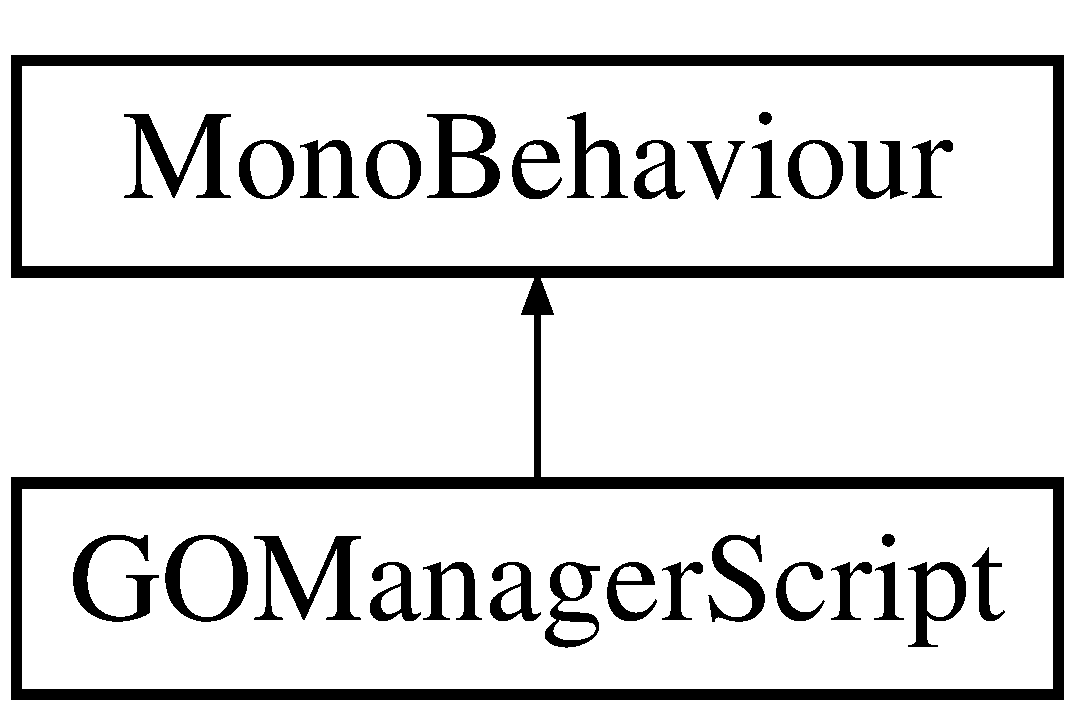
\includegraphics[height=2.000000cm]{class_g_o_manager_script}
\end{center}
\end{figure}
\subsection*{Public Attributes}
\begin{DoxyCompactItemize}
\item 
Text \hyperlink{class_g_o_manager_script_ae6df0f7858c9b610f96af2e6bc84dcad}{score\+Text}
\end{DoxyCompactItemize}
\subsection*{Private Member Functions}
\begin{DoxyCompactItemize}
\item 
void \hyperlink{class_g_o_manager_script_ad493e0419dd25ba9aa8f6945340c1711}{Start} ()
\end{DoxyCompactItemize}


\subsection{Detailed Description}
This script is used to manage the score in the game over screen. 

\subsection{Member Function Documentation}
\hypertarget{class_g_o_manager_script_ad493e0419dd25ba9aa8f6945340c1711}{}\index{G\+O\+Manager\+Script@{G\+O\+Manager\+Script}!Start@{Start}}
\index{Start@{Start}!G\+O\+Manager\+Script@{G\+O\+Manager\+Script}}
\subsubsection[{Start}]{\setlength{\rightskip}{0pt plus 5cm}void G\+O\+Manager\+Script.\+Start (
\begin{DoxyParamCaption}
{}
\end{DoxyParamCaption}
)\hspace{0.3cm}{\ttfamily [inline]}, {\ttfamily [private]}}\label{class_g_o_manager_script_ad493e0419dd25ba9aa8f6945340c1711}
This function is called when the script is first enabled and prints the score. 

\subsection{Member Data Documentation}
\hypertarget{class_g_o_manager_script_ae6df0f7858c9b610f96af2e6bc84dcad}{}\index{G\+O\+Manager\+Script@{G\+O\+Manager\+Script}!score\+Text@{score\+Text}}
\index{score\+Text@{score\+Text}!G\+O\+Manager\+Script@{G\+O\+Manager\+Script}}
\subsubsection[{score\+Text}]{\setlength{\rightskip}{0pt plus 5cm}Text G\+O\+Manager\+Script.\+score\+Text}\label{class_g_o_manager_script_ae6df0f7858c9b610f96af2e6bc84dcad}
The text field in which the score will be printed. 

The documentation for this class was generated from the following file\+:\begin{DoxyCompactItemize}
\item 
A\+O\+T2/\+Assets/\+Scripts/\hyperlink{_g_o_manager_script_8cs}{G\+O\+Manager\+Script.\+cs}\end{DoxyCompactItemize}

\hypertarget{classhand_script}{\section{hand\-Script Class Reference}
\label{classhand_script}\index{hand\-Script@{hand\-Script}}
}
Inheritance diagram for hand\-Script\-:\begin{figure}[H]
\begin{center}
\leavevmode
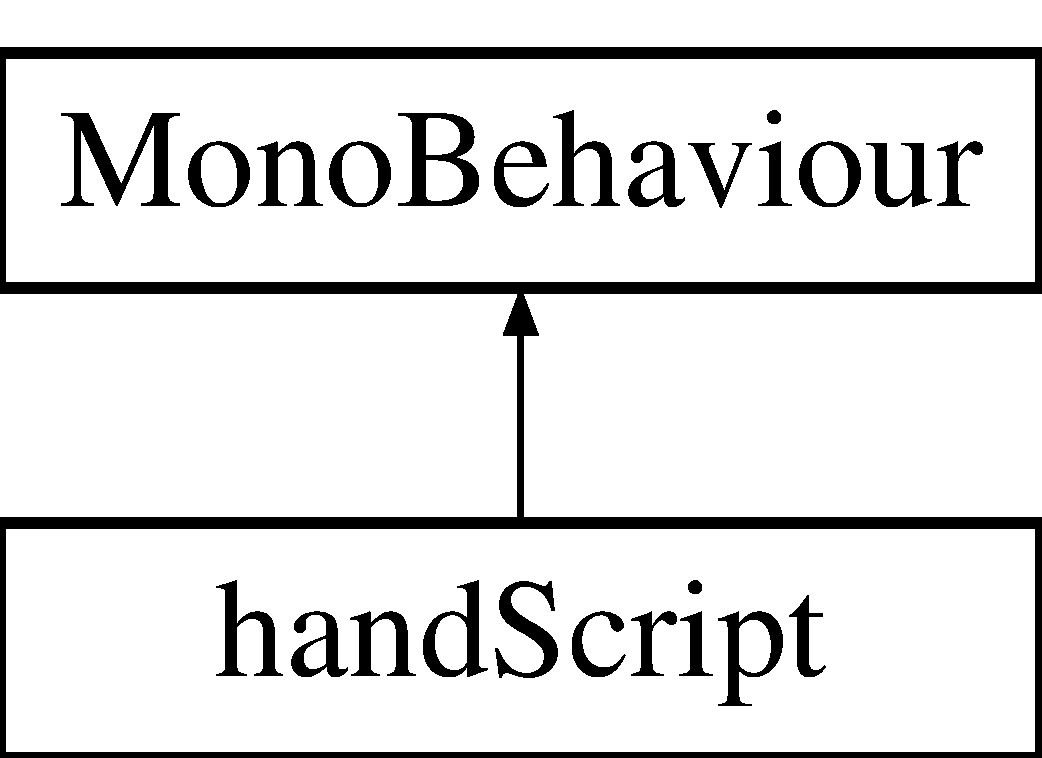
\includegraphics[height=2.000000cm]{classhand_script}
\end{center}
\end{figure}
\subsection*{Public Member Functions}
\begin{DoxyCompactItemize}
\item 
void \hyperlink{classhand_script_a62e593760441c466a04fd26d536cb67a}{L\-H} ()
\item 
void \hyperlink{classhand_script_a64481676bd93e645bed1e263edade065}{R\-H} ()
\end{DoxyCompactItemize}
\subsection*{Public Attributes}
\begin{DoxyCompactItemize}
\item 
Text \hyperlink{classhand_script_a2f300212a9a7f2528c525060eb9d17e4}{this\-Text}
\item 
Text \hyperlink{classhand_script_a2e323ace258263f11a78df53dd7644bd}{other\-Text}
\end{DoxyCompactItemize}
\subsection*{Static Public Attributes}
\begin{DoxyCompactItemize}
\item 
static int \hyperlink{classhand_script_a6ead5b70e39c2831d69fdab64c1226ff}{hand}
\end{DoxyCompactItemize}
\subsection*{Private Member Functions}
\begin{DoxyCompactItemize}
\item 
void \hyperlink{classhand_script_a17986f73e63381c246a9b4b453278fc7}{Start} ()
\item 
void \hyperlink{classhand_script_ac872a547fa3bf7c1a9c800c8d9bdff67}{color\-Changes} ()
\end{DoxyCompactItemize}


\subsection{Detailed Description}
This script handles the handedness of the game. The player can choose left handedness or right handedness. 

\subsection{Member Function Documentation}
\hypertarget{classhand_script_ac872a547fa3bf7c1a9c800c8d9bdff67}{\index{hand\-Script@{hand\-Script}!color\-Changes@{color\-Changes}}
\index{color\-Changes@{color\-Changes}!handScript@{hand\-Script}}
\subsubsection[{color\-Changes}]{\setlength{\rightskip}{0pt plus 5cm}void hand\-Script.\-color\-Changes (
\begin{DoxyParamCaption}
{}
\end{DoxyParamCaption}
)\hspace{0.3cm}{\ttfamily [inline]}, {\ttfamily [private]}}}\label{classhand_script_ac872a547fa3bf7c1a9c800c8d9bdff67}
This function changes the colors of the text, blue for the selected text and white for the other. \hypertarget{classhand_script_a62e593760441c466a04fd26d536cb67a}{\index{hand\-Script@{hand\-Script}!L\-H@{L\-H}}
\index{L\-H@{L\-H}!handScript@{hand\-Script}}
\subsubsection[{L\-H}]{\setlength{\rightskip}{0pt plus 5cm}void hand\-Script.\-L\-H (
\begin{DoxyParamCaption}
{}
\end{DoxyParamCaption}
)\hspace{0.3cm}{\ttfamily [inline]}}}\label{classhand_script_a62e593760441c466a04fd26d536cb67a}
This function is called when L\-H text is clicked and sets the handedness to L\-H. The hand variable is set to 1(L\-H) and the text color is changed. \hypertarget{classhand_script_a64481676bd93e645bed1e263edade065}{\index{hand\-Script@{hand\-Script}!R\-H@{R\-H}}
\index{R\-H@{R\-H}!handScript@{hand\-Script}}
\subsubsection[{R\-H}]{\setlength{\rightskip}{0pt plus 5cm}void hand\-Script.\-R\-H (
\begin{DoxyParamCaption}
{}
\end{DoxyParamCaption}
)\hspace{0.3cm}{\ttfamily [inline]}}}\label{classhand_script_a64481676bd93e645bed1e263edade065}
This function is called when R\-H text is clicked and sets the handedness to R\-H. The hand variable is set to 2(R\-H) and the text color is changed. \hypertarget{classhand_script_a17986f73e63381c246a9b4b453278fc7}{\index{hand\-Script@{hand\-Script}!Start@{Start}}
\index{Start@{Start}!handScript@{hand\-Script}}
\subsubsection[{Start}]{\setlength{\rightskip}{0pt plus 5cm}void hand\-Script.\-Start (
\begin{DoxyParamCaption}
{}
\end{DoxyParamCaption}
)\hspace{0.3cm}{\ttfamily [inline]}, {\ttfamily [private]}}}\label{classhand_script_a17986f73e63381c246a9b4b453278fc7}
This function is called when the script is first enabled. The default handedness(right handed) is set in this function. 

\subsection{Member Data Documentation}
\hypertarget{classhand_script_a6ead5b70e39c2831d69fdab64c1226ff}{\index{hand\-Script@{hand\-Script}!hand@{hand}}
\index{hand@{hand}!handScript@{hand\-Script}}
\subsubsection[{hand}]{\setlength{\rightskip}{0pt plus 5cm}int hand\-Script.\-hand\hspace{0.3cm}{\ttfamily [static]}}}\label{classhand_script_a6ead5b70e39c2831d69fdab64c1226ff}
The variable that stores the chosen handedness of the player. \hypertarget{classhand_script_a2e323ace258263f11a78df53dd7644bd}{\index{hand\-Script@{hand\-Script}!other\-Text@{other\-Text}}
\index{other\-Text@{other\-Text}!handScript@{hand\-Script}}
\subsubsection[{other\-Text}]{\setlength{\rightskip}{0pt plus 5cm}Text hand\-Script.\-other\-Text}}\label{classhand_script_a2e323ace258263f11a78df53dd7644bd}
The text field that does not use this instance of the script (L\-H or R\-H) \hypertarget{classhand_script_a2f300212a9a7f2528c525060eb9d17e4}{\index{hand\-Script@{hand\-Script}!this\-Text@{this\-Text}}
\index{this\-Text@{this\-Text}!handScript@{hand\-Script}}
\subsubsection[{this\-Text}]{\setlength{\rightskip}{0pt plus 5cm}Text hand\-Script.\-this\-Text}}\label{classhand_script_a2f300212a9a7f2528c525060eb9d17e4}
The text field that uses this instance of the script (L\-H or R\-H) 

The documentation for this class was generated from the following file\-:\begin{DoxyCompactItemize}
\item 
A\-O\-T2/\-Assets/\-Scripts/\hyperlink{hand_script_8cs}{hand\-Script.\-cs}\end{DoxyCompactItemize}

\hypertarget{class_manager_scrip}{}\section{Manager\+Scrip Class Reference}
\label{class_manager_scrip}\index{Manager\+Scrip@{Manager\+Scrip}}
Inheritance diagram for Manager\+Scrip\+:\begin{figure}[H]
\begin{center}
\leavevmode
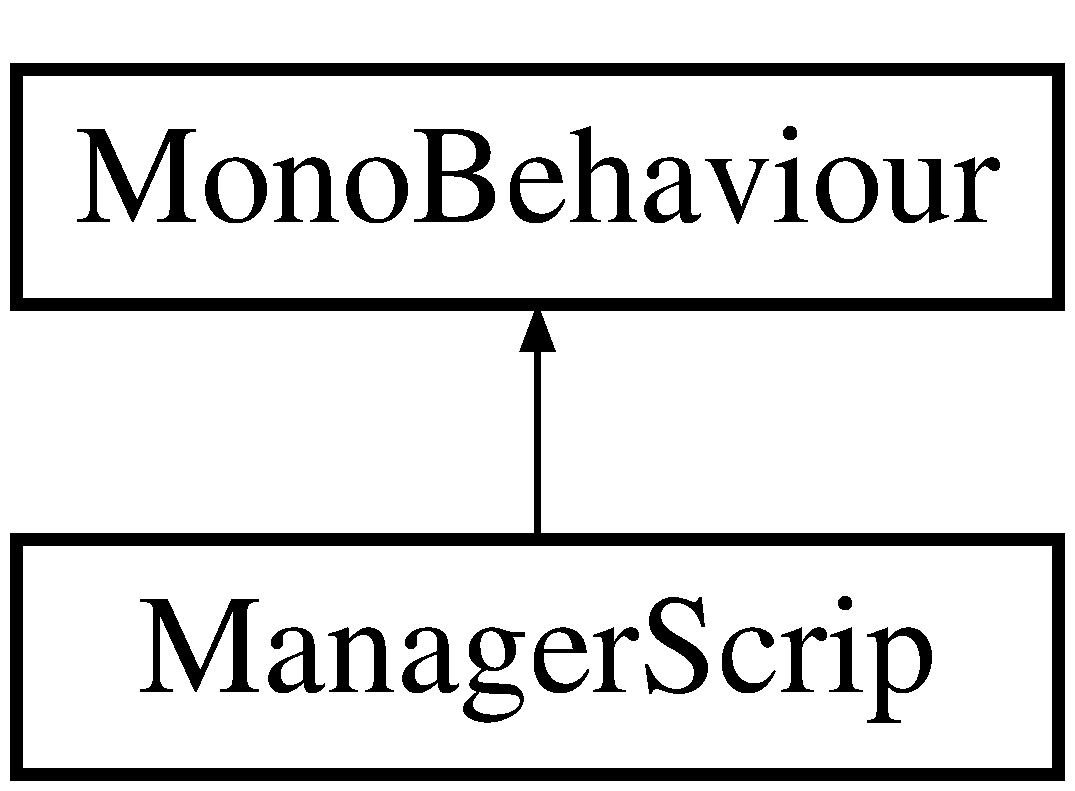
\includegraphics[height=2.000000cm]{class_manager_scrip}
\end{center}
\end{figure}
\subsection*{Public Member Functions}
\begin{DoxyCompactItemize}
\item 
\hypertarget{class_manager_scrip_a44177d26694eced8c1f72ba14ba9b0a6}{}void {\bfseries Add\+Score} (int x)\label{class_manager_scrip_a44177d26694eced8c1f72ba14ba9b0a6}

\end{DoxyCompactItemize}
\subsection*{Public Attributes}
\begin{DoxyCompactItemize}
\item 
\hypertarget{class_manager_scrip_a08b542ecf690456e3dad0aa2824cac1a}{}G\+U\+I\+Text {\bfseries score\+Text}\label{class_manager_scrip_a08b542ecf690456e3dad0aa2824cac1a}

\end{DoxyCompactItemize}
\subsection*{Static Public Attributes}
\begin{DoxyCompactItemize}
\item 
\hypertarget{class_manager_scrip_ab1fd8dd95add5e61275e511e72f8e94d}{}static int {\bfseries tot\+Score\+Int}\label{class_manager_scrip_ab1fd8dd95add5e61275e511e72f8e94d}

\end{DoxyCompactItemize}


The documentation for this class was generated from the following file\+:\begin{DoxyCompactItemize}
\item 
A\+O\+T2/\+Assets/\+Scripts/Manager\+Scrip.\+cs\end{DoxyCompactItemize}

\hypertarget{class_pause_menu}{}\section{Pause\+Menu Class Reference}
\label{class_pause_menu}\index{Pause\+Menu@{Pause\+Menu}}
Inheritance diagram for Pause\+Menu\+:\begin{figure}[H]
\begin{center}
\leavevmode
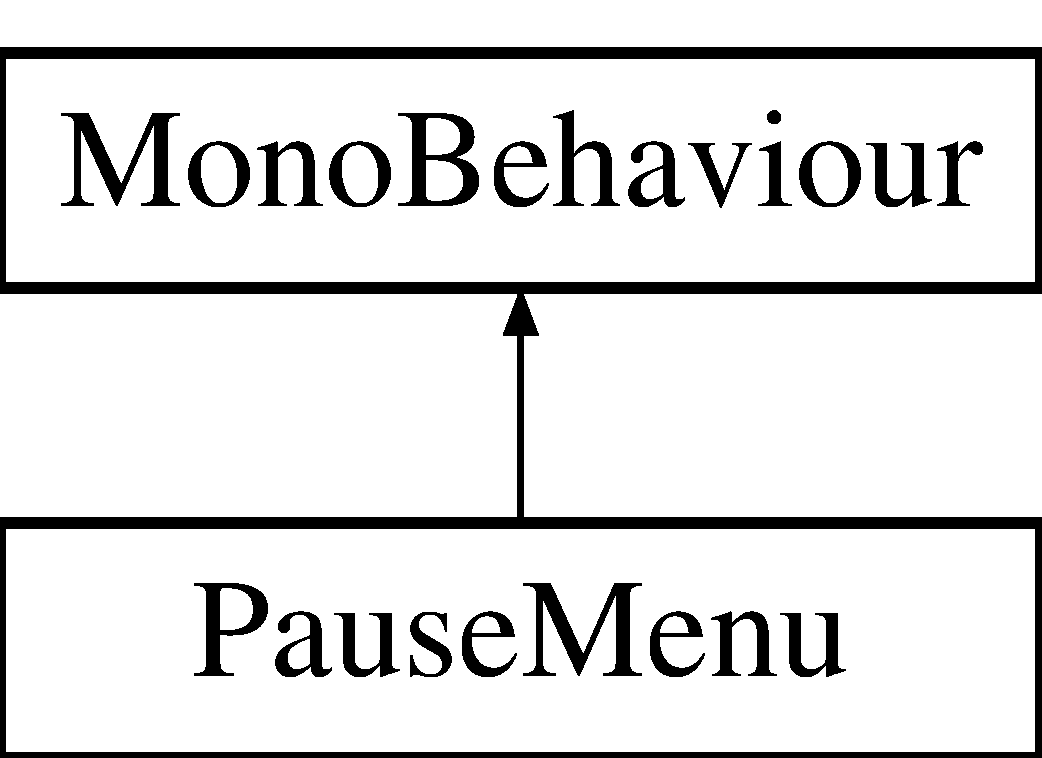
\includegraphics[height=2.000000cm]{class_pause_menu}
\end{center}
\end{figure}
\subsection*{Public Attributes}
\begin{DoxyCompactItemize}
\item 
G\+U\+I\+Skin \hyperlink{class_pause_menu_af78d9844a86f8ffb0ebf4d711fe0c2ce}{my\+Skin}
\end{DoxyCompactItemize}


\subsection{Member Data Documentation}
\hypertarget{class_pause_menu_af78d9844a86f8ffb0ebf4d711fe0c2ce}{}\index{Pause\+Menu@{Pause\+Menu}!my\+Skin@{my\+Skin}}
\index{my\+Skin@{my\+Skin}!Pause\+Menu@{Pause\+Menu}}
\subsubsection[{my\+Skin}]{\setlength{\rightskip}{0pt plus 5cm}G\+U\+I\+Skin Pause\+Menu.\+my\+Skin}\label{class_pause_menu_af78d9844a86f8ffb0ebf4d711fe0c2ce}
\hyperlink{class_pause_menu}{Pause\+Menu} script allows the Pause Interface to enable the user to access settings that may need to be changed mid-\/game. In addition, the player can pause to take a break during a game. 

The documentation for this class was generated from the following file\+:\begin{DoxyCompactItemize}
\item 
A\+O\+T2/\+Assets/\+Scripts/Pause\+Menu.\+cs\end{DoxyCompactItemize}

\hypertarget{classshooter_script}{}\section{shooter\+Script Class Reference}
\label{classshooter_script}\index{shooter\+Script@{shooter\+Script}}
Inheritance diagram for shooter\+Script\+:\begin{figure}[H]
\begin{center}
\leavevmode
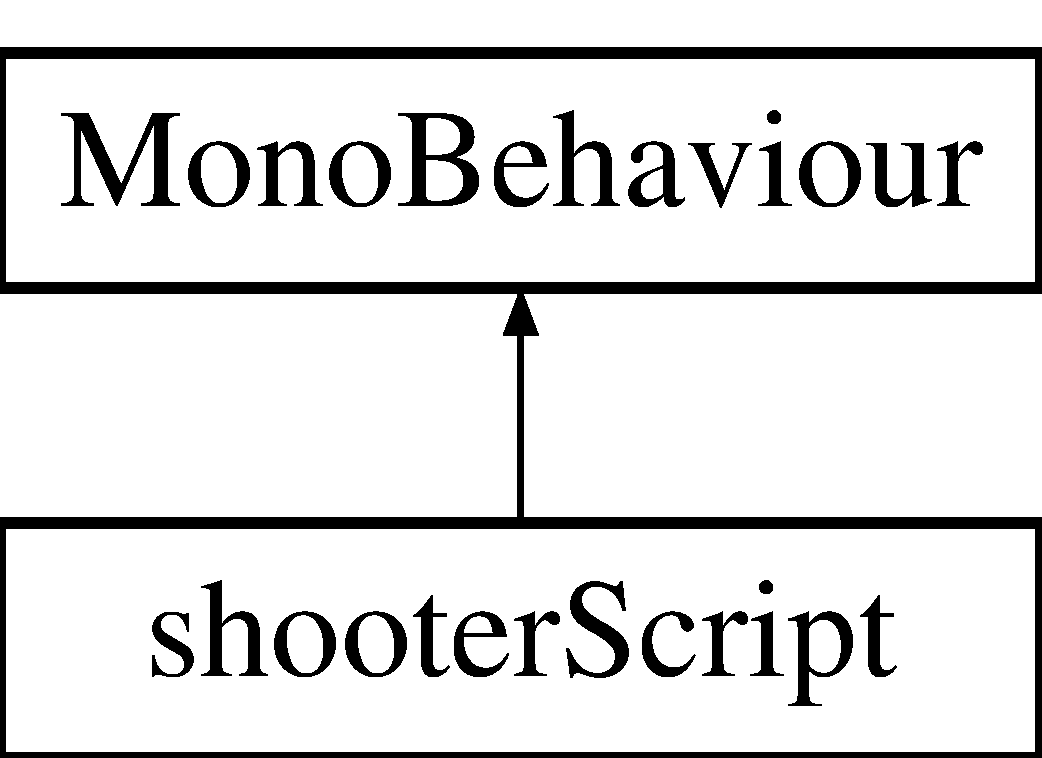
\includegraphics[height=2.000000cm]{classshooter_script}
\end{center}
\end{figure}
\subsection*{Public Attributes}
\begin{DoxyCompactItemize}
\item 
Game\+Object \hyperlink{classshooter_script_aec5b91ec83c6e5326f9f251f46411367}{Circle}
\item 
float \hyperlink{classshooter_script_a35395b1d291048e31353f9300c4e61be}{shoot\+Lim}
\end{DoxyCompactItemize}
\subsection*{Private Member Functions}
\begin{DoxyCompactItemize}
\item 
void \hyperlink{classshooter_script_a5537eb84985ee1bd03183f66b4f87237}{Start} ()
\item 
void \hyperlink{classshooter_script_a4076123ad3efc3184b433ec934cce1bd}{Update} ()
\end{DoxyCompactItemize}
\subsection*{Private Attributes}
\begin{DoxyCompactItemize}
\item 
float \hyperlink{classshooter_script_a3b49886ffefc2a63ad5cb5995da709b4}{last\+Shot}
\end{DoxyCompactItemize}


\subsection{Member Function Documentation}
\hypertarget{classshooter_script_a5537eb84985ee1bd03183f66b4f87237}{}\index{shooter\+Script@{shooter\+Script}!Start@{Start}}
\index{Start@{Start}!shooter\+Script@{shooter\+Script}}
\subsubsection[{Start}]{\setlength{\rightskip}{0pt plus 5cm}void shooter\+Script.\+Start (
\begin{DoxyParamCaption}
{}
\end{DoxyParamCaption}
)\hspace{0.3cm}{\ttfamily [inline]}, {\ttfamily [private]}}\label{classshooter_script_a5537eb84985ee1bd03183f66b4f87237}
Limit the speed that projectiles can be shot. \hypertarget{classshooter_script_a4076123ad3efc3184b433ec934cce1bd}{}\index{shooter\+Script@{shooter\+Script}!Update@{Update}}
\index{Update@{Update}!shooter\+Script@{shooter\+Script}}
\subsubsection[{Update}]{\setlength{\rightskip}{0pt plus 5cm}void shooter\+Script.\+Update (
\begin{DoxyParamCaption}
{}
\end{DoxyParamCaption}
)\hspace{0.3cm}{\ttfamily [inline]}, {\ttfamily [private]}}\label{classshooter_script_a4076123ad3efc3184b433ec934cce1bd}
If user clicks mouse in the bounded area, fire projectiles.

x and y coordinates are used to ensure projectiles can only be fired from the bar.

Ensure that the rate of fire is limited. 

\subsection{Member Data Documentation}
\hypertarget{classshooter_script_aec5b91ec83c6e5326f9f251f46411367}{}\index{shooter\+Script@{shooter\+Script}!Circle@{Circle}}
\index{Circle@{Circle}!shooter\+Script@{shooter\+Script}}
\subsubsection[{Circle}]{\setlength{\rightskip}{0pt plus 5cm}Game\+Object shooter\+Script.\+Circle}\label{classshooter_script_aec5b91ec83c6e5326f9f251f46411367}
This script allows projectiles to be fired within the shooter bar on the left or right of the screen. Position coordinates are used to ensure that projectiles are only able to be fired from the shooter bar. \hypertarget{classshooter_script_a3b49886ffefc2a63ad5cb5995da709b4}{}\index{shooter\+Script@{shooter\+Script}!last\+Shot@{last\+Shot}}
\index{last\+Shot@{last\+Shot}!shooter\+Script@{shooter\+Script}}
\subsubsection[{last\+Shot}]{\setlength{\rightskip}{0pt plus 5cm}float shooter\+Script.\+last\+Shot\hspace{0.3cm}{\ttfamily [private]}}\label{classshooter_script_a3b49886ffefc2a63ad5cb5995da709b4}
\hypertarget{classshooter_script_a35395b1d291048e31353f9300c4e61be}{}\index{shooter\+Script@{shooter\+Script}!shoot\+Lim@{shoot\+Lim}}
\index{shoot\+Lim@{shoot\+Lim}!shooter\+Script@{shooter\+Script}}
\subsubsection[{shoot\+Lim}]{\setlength{\rightskip}{0pt plus 5cm}float shooter\+Script.\+shoot\+Lim}\label{classshooter_script_a35395b1d291048e31353f9300c4e61be}


The documentation for this class was generated from the following file\+:\begin{DoxyCompactItemize}
\item 
A\+O\+T2/\+Assets/\+Scripts/\hyperlink{shooter_script_8cs}{shooter\+Script.\+cs}\end{DoxyCompactItemize}

\hypertarget{classspawner_script}{}\section{spawner\+Script Class Reference}
\label{classspawner_script}\index{spawner\+Script@{spawner\+Script}}
Inheritance diagram for spawner\+Script\+:\begin{figure}[H]
\begin{center}
\leavevmode
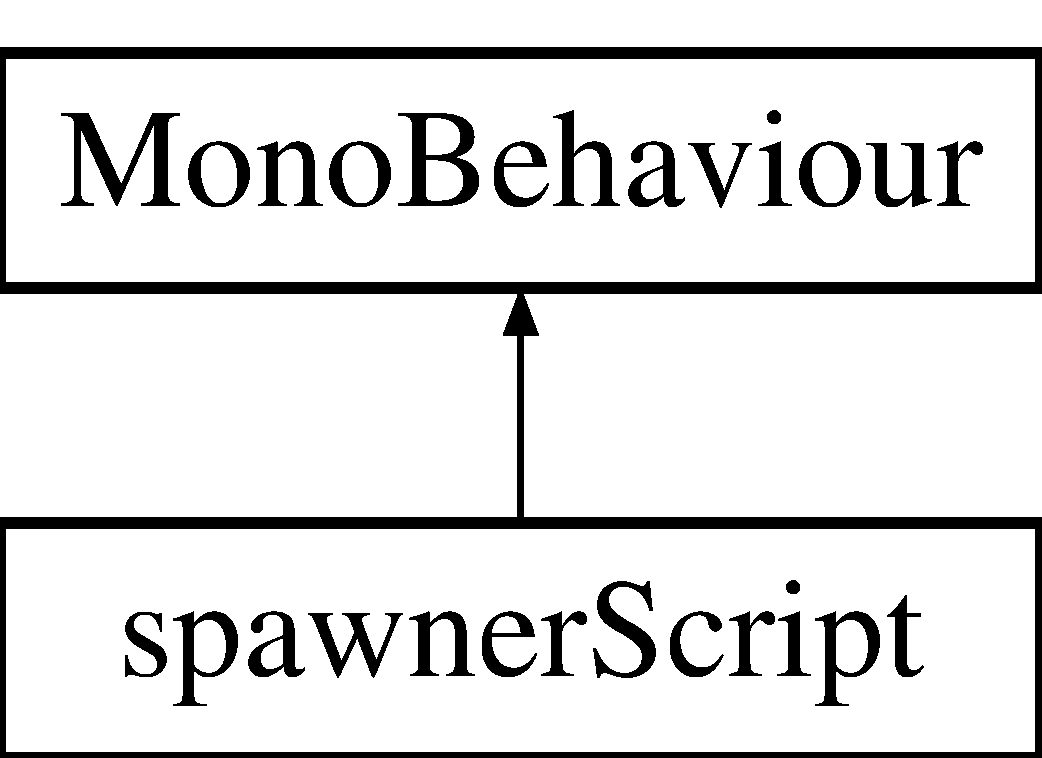
\includegraphics[height=2.000000cm]{classspawner_script}
\end{center}
\end{figure}
\subsection*{Public Attributes}
\begin{DoxyCompactItemize}
\item 
float \hyperlink{classspawner_script_a93800079e4f6fcd8728db3d0735aba79}{spawnt} = 1
\item 
Game\+Object \hyperlink{classspawner_script_ad99dc33b3262b1bb666846d952e5e0f4}{Triangle}
\begin{DoxyCompactList}\small\item\em Controls rate at which triangles spawn. \end{DoxyCompactList}\end{DoxyCompactItemize}
\subsection*{Private Member Functions}
\begin{DoxyCompactItemize}
\item 
void \hyperlink{classspawner_script_a51f0da0f6ec9342ee86ea7888d66fff8}{Start} ()
\item 
void \hyperlink{classspawner_script_a485b56d5b5d75b842e568d839aaaaa7e}{new\+Triangle} ()
\begin{DoxyCompactList}\small\item\em The following method controls where the triangles spawn. \end{DoxyCompactList}\end{DoxyCompactItemize}


\subsection{Member Function Documentation}
\hypertarget{classspawner_script_a485b56d5b5d75b842e568d839aaaaa7e}{}\index{spawner\+Script@{spawner\+Script}!new\+Triangle@{new\+Triangle}}
\index{new\+Triangle@{new\+Triangle}!spawner\+Script@{spawner\+Script}}
\subsubsection[{new\+Triangle}]{\setlength{\rightskip}{0pt plus 5cm}void spawner\+Script.\+new\+Triangle (
\begin{DoxyParamCaption}
{}
\end{DoxyParamCaption}
)\hspace{0.3cm}{\ttfamily [inline]}, {\ttfamily [private]}}\label{classspawner_script_a485b56d5b5d75b842e568d839aaaaa7e}


The following method controls where the triangles spawn. 

Spawn many instances of enemy triangles. \hypertarget{classspawner_script_a51f0da0f6ec9342ee86ea7888d66fff8}{}\index{spawner\+Script@{spawner\+Script}!Start@{Start}}
\index{Start@{Start}!spawner\+Script@{spawner\+Script}}
\subsubsection[{Start}]{\setlength{\rightskip}{0pt plus 5cm}void spawner\+Script.\+Start (
\begin{DoxyParamCaption}
{}
\end{DoxyParamCaption}
)\hspace{0.3cm}{\ttfamily [inline]}, {\ttfamily [private]}}\label{classspawner_script_a51f0da0f6ec9342ee86ea7888d66fff8}
Triangle game objects will spawn repeatedly. 

\subsection{Member Data Documentation}
\hypertarget{classspawner_script_a93800079e4f6fcd8728db3d0735aba79}{}\index{spawner\+Script@{spawner\+Script}!spawnt@{spawnt}}
\index{spawnt@{spawnt}!spawner\+Script@{spawner\+Script}}
\subsubsection[{spawnt}]{\setlength{\rightskip}{0pt plus 5cm}float spawner\+Script.\+spawnt = 1}\label{classspawner_script_a93800079e4f6fcd8728db3d0735aba79}
This script spawns instances of the enemy triangles so that the user can shoot the triangles to defend the squares below. \hypertarget{classspawner_script_ad99dc33b3262b1bb666846d952e5e0f4}{}\index{spawner\+Script@{spawner\+Script}!Triangle@{Triangle}}
\index{Triangle@{Triangle}!spawner\+Script@{spawner\+Script}}
\subsubsection[{Triangle}]{\setlength{\rightskip}{0pt plus 5cm}Game\+Object spawner\+Script.\+Triangle}\label{classspawner_script_ad99dc33b3262b1bb666846d952e5e0f4}


Controls rate at which triangles spawn. 



The documentation for this class was generated from the following file\+:\begin{DoxyCompactItemize}
\item 
A\+O\+T2/\+Assets/\+Scripts/\hyperlink{spawner_script_8cs}{spawner\+Script.\+cs}\end{DoxyCompactItemize}

\hypertarget{classsquare_script}{}\section{square\+Script Class Reference}
\label{classsquare_script}\index{square\+Script@{square\+Script}}
Inheritance diagram for square\+Script\+:\begin{figure}[H]
\begin{center}
\leavevmode
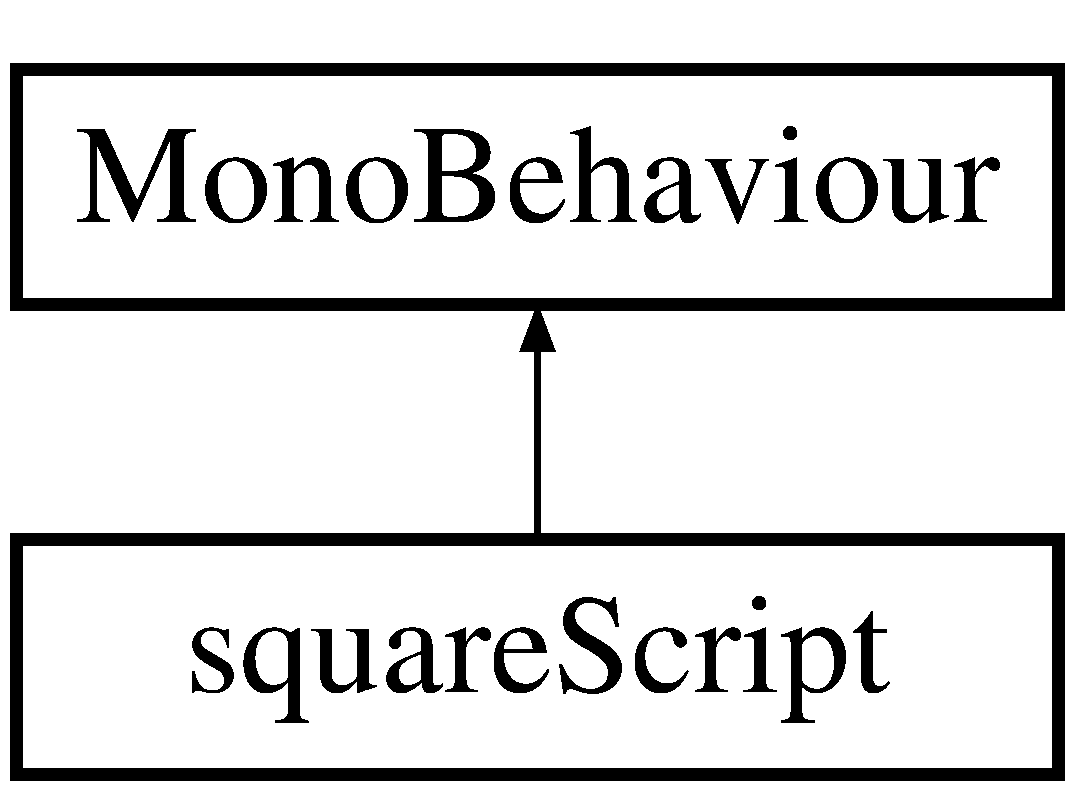
\includegraphics[height=2.000000cm]{classsquare_script}
\end{center}
\end{figure}
\subsection*{Public Member Functions}
\begin{DoxyCompactItemize}
\item 
void \hyperlink{classsquare_script_a63e48b93a844b2a14c3e3a691165d8fb}{On\+Trigger\+Enter2\+D} (Collider2\+D obj)
\end{DoxyCompactItemize}


\subsection{Detailed Description}
This script is used by the Square objects in the game. This script deals with the collision detection of the Square objects. 

\subsection{Member Function Documentation}
\hypertarget{classsquare_script_a63e48b93a844b2a14c3e3a691165d8fb}{}\index{square\+Script@{square\+Script}!On\+Trigger\+Enter2\+D@{On\+Trigger\+Enter2\+D}}
\index{On\+Trigger\+Enter2\+D@{On\+Trigger\+Enter2\+D}!square\+Script@{square\+Script}}
\subsubsection[{On\+Trigger\+Enter2\+D}]{\setlength{\rightskip}{0pt plus 5cm}void square\+Script.\+On\+Trigger\+Enter2\+D (
\begin{DoxyParamCaption}
\item[{Collider2\+D}]{obj}
\end{DoxyParamCaption}
)\hspace{0.3cm}{\ttfamily [inline]}}\label{classsquare_script_a63e48b93a844b2a14c3e3a691165d8fb}
This function handles the collision detection of the Square objects. This function is called when a collision with a Square object is detected. Handles removal of both Circle and Triangle objects, only removing the Square object when a collision with a Triangle occurs. 
\begin{DoxyParams}{Parameters}
{\em obj} & the object that collided with the Square \\
\hline
\end{DoxyParams}


The documentation for this class was generated from the following file\+:\begin{DoxyCompactItemize}
\item 
A\+O\+T2/\+Assets/\+Scripts/\hyperlink{square_script_8cs}{square\+Script.\+cs}\end{DoxyCompactItemize}

\hypertarget{classsquare_spawn_script}{}\section{square\+Spawn\+Script Class Reference}
\label{classsquare_spawn_script}\index{square\+Spawn\+Script@{square\+Spawn\+Script}}
Inheritance diagram for square\+Spawn\+Script\+:\begin{figure}[H]
\begin{center}
\leavevmode
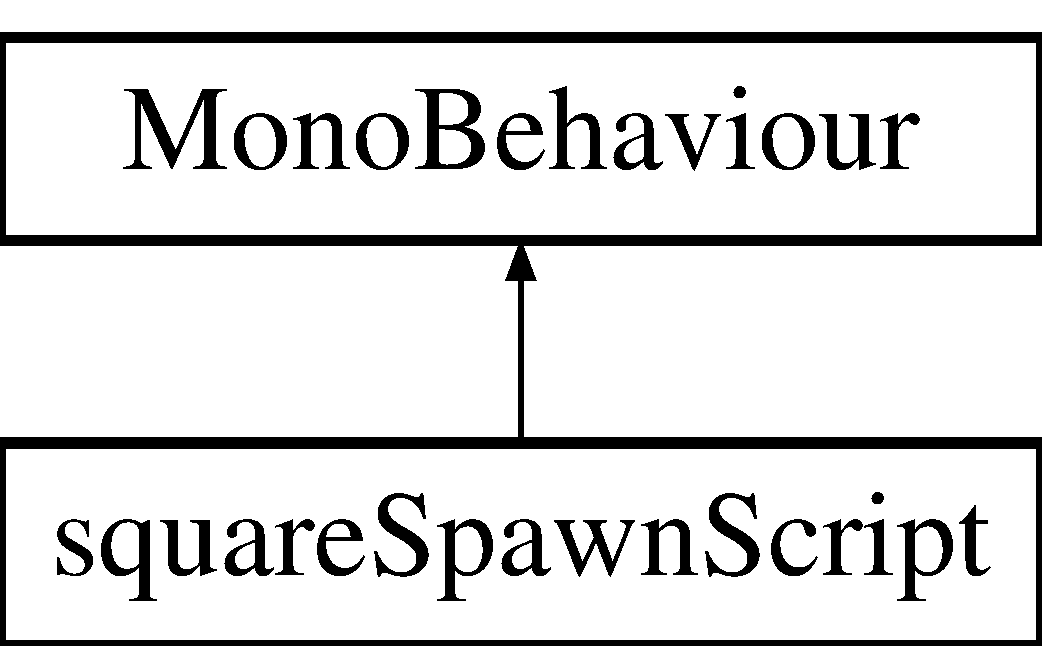
\includegraphics[height=2.000000cm]{classsquare_spawn_script}
\end{center}
\end{figure}
\subsection*{Public Member Functions}
\begin{DoxyCompactItemize}
\item 
\hypertarget{classsquare_spawn_script_a072454e82d37b10169a363717acfc2be}{}void {\bfseries On\+Trigger\+Enter2\+D} (Collider2\+D obj)\label{classsquare_spawn_script_a072454e82d37b10169a363717acfc2be}

\end{DoxyCompactItemize}
\subsection*{Public Attributes}
\begin{DoxyCompactItemize}
\item 
\hypertarget{classsquare_spawn_script_a353637659973cde399b46b194b30eb2e}{}Game\+Object {\bfseries squares}\label{classsquare_spawn_script_a353637659973cde399b46b194b30eb2e}

\item 
\hypertarget{classsquare_spawn_script_aee81b01036a29f961a113a21183173e3}{}int {\bfseries numsquares}\label{classsquare_spawn_script_aee81b01036a29f961a113a21183173e3}

\item 
\hypertarget{classsquare_spawn_script_acc39770a5d684a4b5e1057b832dc979d}{}Camera {\bfseries R\+H}\label{classsquare_spawn_script_acc39770a5d684a4b5e1057b832dc979d}

\item 
\hypertarget{classsquare_spawn_script_abf8f64837c29453bfe6231d48b06b483}{}Camera {\bfseries L\+H}\label{classsquare_spawn_script_abf8f64837c29453bfe6231d48b06b483}

\end{DoxyCompactItemize}


The documentation for this class was generated from the following file\+:\begin{DoxyCompactItemize}
\item 
A\+O\+T2/\+Assets/\+Scripts/square\+Spawn\+Script.\+cs\end{DoxyCompactItemize}

\hypertarget{classtriangle_script}{}\section{triangle\+Script Class Reference}
\label{classtriangle_script}\index{triangle\+Script@{triangle\+Script}}
Inheritance diagram for triangle\+Script\+:\begin{figure}[H]
\begin{center}
\leavevmode
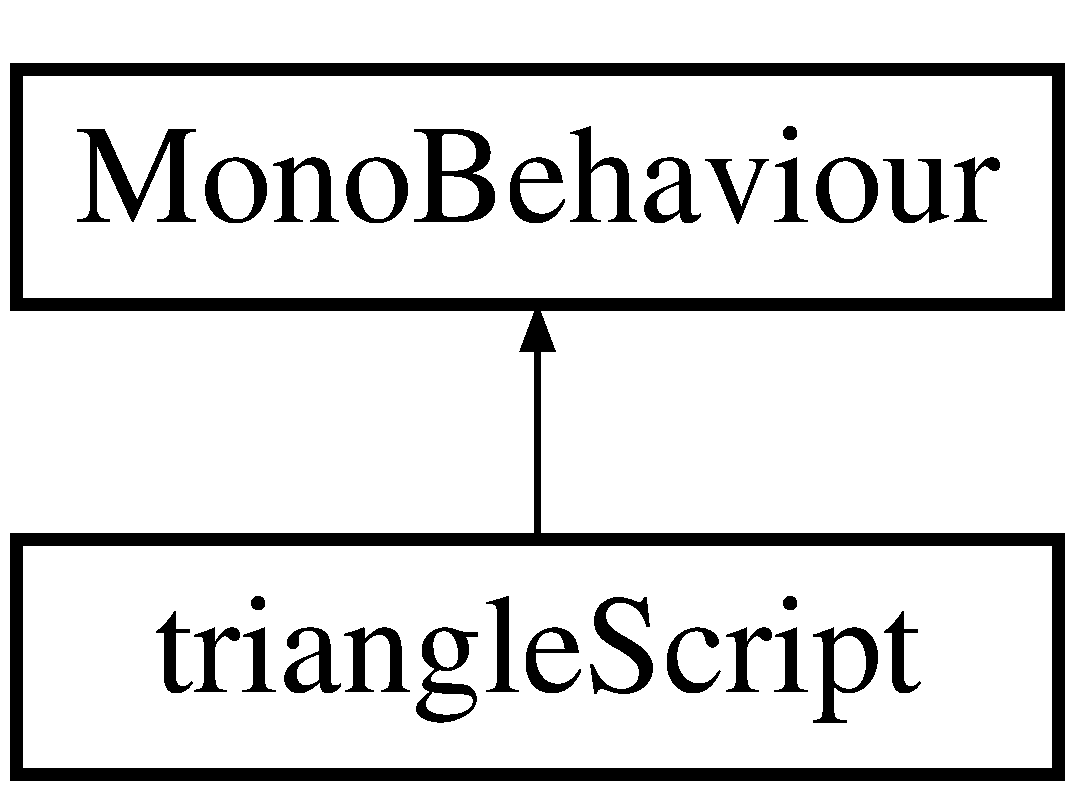
\includegraphics[height=2.000000cm]{classtriangle_script}
\end{center}
\end{figure}
\subsection*{Public Member Functions}
\begin{DoxyCompactItemize}
\item 
void \hyperlink{classtriangle_script_a6deb98a0bb688a322a75d03e61e6e5e8}{On\+Became\+Invisible} ()
\end{DoxyCompactItemize}
\subsection*{Public Attributes}
\begin{DoxyCompactItemize}
\item 
Vector2 \hyperlink{classtriangle_script_a6bfdbe74d4572da3bac0362003649747}{speed}
\end{DoxyCompactItemize}
\subsection*{Private Member Functions}
\begin{DoxyCompactItemize}
\item 
void \hyperlink{classtriangle_script_ab63e77d33e9bd070628898b9926a7dad}{Start} ()
\end{DoxyCompactItemize}


\subsection{Detailed Description}
Script that is used by the Triangle objects in the game. The script handles the Triangle objects, particularly their speeds and their destruction on exiting the screen. 

\subsection{Member Function Documentation}
\hypertarget{classtriangle_script_a6deb98a0bb688a322a75d03e61e6e5e8}{}\index{triangle\+Script@{triangle\+Script}!On\+Became\+Invisible@{On\+Became\+Invisible}}
\index{On\+Became\+Invisible@{On\+Became\+Invisible}!triangle\+Script@{triangle\+Script}}
\subsubsection[{On\+Became\+Invisible}]{\setlength{\rightskip}{0pt plus 5cm}void triangle\+Script.\+On\+Became\+Invisible (
\begin{DoxyParamCaption}
{}
\end{DoxyParamCaption}
)\hspace{0.3cm}{\ttfamily [inline]}}\label{classtriangle_script_a6deb98a0bb688a322a75d03e61e6e5e8}
Function that is run when object that uses \hyperlink{classtriangle_script}{triangle\+Script} leaves the screen. If the Triangle object exits the screen, it is destroyed. \hypertarget{classtriangle_script_ab63e77d33e9bd070628898b9926a7dad}{}\index{triangle\+Script@{triangle\+Script}!Start@{Start}}
\index{Start@{Start}!triangle\+Script@{triangle\+Script}}
\subsubsection[{Start}]{\setlength{\rightskip}{0pt plus 5cm}void triangle\+Script.\+Start (
\begin{DoxyParamCaption}
{}
\end{DoxyParamCaption}
)\hspace{0.3cm}{\ttfamily [inline]}, {\ttfamily [private]}}\label{classtriangle_script_ab63e77d33e9bd070628898b9926a7dad}
Initializer for \hyperlink{classtriangle_script}{triangle\+Script}. This is run when the script is first enabled. Speed is assigned to the Triangle objects depending on the difficulty chosen. 

\subsection{Member Data Documentation}
\hypertarget{classtriangle_script_a6bfdbe74d4572da3bac0362003649747}{}\index{triangle\+Script@{triangle\+Script}!speed@{speed}}
\index{speed@{speed}!triangle\+Script@{triangle\+Script}}
\subsubsection[{speed}]{\setlength{\rightskip}{0pt plus 5cm}Vector2 triangle\+Script.\+speed}\label{classtriangle_script_a6bfdbe74d4572da3bac0362003649747}
The vector that the Triangle object\textquotesingle{}s velocity will be set to. 

The documentation for this class was generated from the following file\+:\begin{DoxyCompactItemize}
\item 
A\+O\+T2/\+Assets/\+Scripts/\hyperlink{triangle_script_8cs}{triangle\+Script.\+cs}\end{DoxyCompactItemize}

%--- End generated contents ---

% Index
\backmatter
\newpage
\phantomsection
\clearemptydoublepage
\addcontentsline{toc}{chapter}{Index}
\printindex

\end{document}
